%Report for ProbaBLAST
%\documentclass[12pt]{article}%
\documentclass[12pt]{IEEEtran}
\usepackage{setspace}
\onehalfspacing
\usepackage[margin=2.5cm]{geometry}
\usepackage{amsmath}
\usepackage{cite}
\usepackage{amsfonts}
\usepackage{graphicx}
\usepackage{mathptmx}
\usepackage{algpseudocode,algorithm,algorithmicx}
\newcommand*\Let[2]{\State #1 $\gets$ #2}
\algrenewcommand\algorithmicrequire{\textbf{Precondition:}}

\begin{document}

\title{ProbaBLAST: a Probabilistic Approach to Sequence Alignment}
\author{Michael Noseworthy, Pascale Gourdeau}
\date{}
\maketitle

\section{Introduction}

The local sequence alignment problem seems simple: given a sequence query $Q$ and a database sequence $D$, how can we align substrings of $Q$ with substrings in $D$? Moreover, given a certain \emph{scoring scheme}, which pair of substrings achieves the best score? We usually wish to compare a somewhat short sequence of nucleotides against a whole genome. Natually, the two sequences differ in size by many orders of magnitude, and the Smith-Waterman algorithm, which finds an optimal solution, is extremely computationally expensive. 

One of the most well-known and commonly used algorithm in bioinformatics, the Basic Local Alignment Search Tool (BLAST), while not guaranteeing an optimal solution to the local sequence alignment problem, reduces immensely computational time compared to the Smith-Waterman algorithm, while still giving perfectly reasonable answers. It was originally presented in \cite{originalBLAST} and has been improved many times over the years \cite{blast2}. Moreover, different versions of the algorithm have been developed to better respond to specific problems surrounding sequence alignment. 

It is however not always possible to work with a genome for which we know the nucleotides at all positions with certainty. Indeed, it is possible that the genome assembly gave ambigous results at certain positions. Moreover, computationally inferring ancestral sequences, an active branch of research in computational biology, inherently deals with uncertainty. From these two issues arises a probabilistic version of the genome, which is represented as probability matrix with 4 rows, one for each nucleotide, and $L$ columns, where $L$ is the length of the genome. In this case, we cannot use the BLAST algorithm to find local alignments between a deterministic query sequence and a probabilistic database.

This report presents our approach to the problem of probabilistic sequence alignment. 
We first introduce ProbaBLAST, an analog of the BLAST algorithm. We then present and evaluate our algorithm's performance and suggest ways in which to improve it.


\section{Methodology}

There are two heuristics at the basis of the BLAST algorithm:
\begin{enumerate}
\item Most high scoring local alignments contain a high scoring \emph{gapless} subalignment.
\item Most high scoring pairs contain a perfect match of a certain length $w$
\end{enumerate}
These heuristics still hold for our probabilistic version of the sequence alignment problem, and so our algorithm is largely inspired from BLAST. Our modifications include: (i) two possible ways of building an index, and (ii) a modified scoring scheme. If we were to input to ProbaBLAST a deterministic sequence (i.e. a sequence where all the probability mass is assigned to a single nucleotide at each position), we would indeed have the original BLAST algorithm. There is also a need to create a different methodology to evaluate ProbaBLAST, which is presented in the last subsection.

\subsection{Building indices}

We first decided to investigate two different ways to build an index of the genome. This index has $4^w$ entries, each corresponding to a string of nucleotides of lentgh $w$ and their positions in the genome.

The first method is based on maximum likelihood estimates: for each position in the genome, we pick the nucleotide with highest probability. This approach is simple and sound, but we thought it might be too forgiving to cases where the probabilities associated with a series of nucleotides is low.
This is why we decided to create a second type of index. For a given string $x=x_1,\dots,x_n$ in the genome, we index it in the database only if 
$$P(x)=\prod_{i=1}^{n}P(x_i)\geq t^w$$
where $P(x_i)$ is the probability associated with nucleotide at position $i$  and $t$ is a threshold value. Intuitively, we only allow strings of nucleotides for which the average probability is above $t$. We chose threshold values of $0.925$, $0.95$ and $0.975$. They are based on the genome we are testing ProbaBLAST on, i.e. when the index started to differ from the maximum likelihood version of the index.

\subsection{A new scoring scheme}

We also had to modify the scoring scheme used in BLAST. Indeed, if a sequence taken from the genome has a relatively low probability, we should be more skeptical of matches and mismatches. On the other hand, a gap is almost equally significant in both high and low probability sequences: if there is a difference between the true and observed nucleotides at one or two consecutive positions, then it is much more likely that the optimal alignment we will put a mismatch than a gap at this position.

Under the defaults values: $\text{mismatch}= -1$, $\text{match}= 2$ and $\text{gap} = -2$, we have the following updated scoring function:

\begin{algorithm}
  \caption{Alignment score between two sequences
    \label{alg:score}}
  \begin{algorithmic}[1]
 \Require{$S$ and $T$ have the same length. $S$ is probabilitistic, $T$ is deterministic}
    \Statex
    \Function{Score}{$T, S$}
      \Let{$\text{score}$}{$0$}
      \For{$i \gets 1 \textrm{ to } \text{length}(T)$}
        \If{$s_i = t_i$}
          	\Let{$\text{score}$}{$\text{score} + 2\cdot P(s_i)$}
	\ElsIf{$s_i=\text{gap}$ \textbf{or}  $t_i=\text{gap}$}
		\Let{$\text{score}$}{$\text{score} - 2$}
	\Else 
		\Let{$\text{score}$}{$\text{score} - P(s_i)$}
        \EndIf
      \EndFor
      \State \Return{$\text{score}$}
    \EndFunction
  \end{algorithmic}
\end{algorithm}

\subsection{Putting it all together: ProbaBLAST}

The remaining of the algorithm follows the BLAST implementation: we build an index $D$ and for each new query $Q$, we store every perfect match of length $w$ between $Q$ and $D$. These are called the \emph{seeds} and constitute the basis aligning substrings of $Q$ and $D$. Then follows an ungapped extension phase, where we match nucleotides on the edge of the seed and keep track of the new score. We stop we the difference between the current score and the maximum score seen so far exceeds a given threshold. We then check to see if the score of the extended sequence exceeds a threshold $T$. If it does not, we throw away the match. 

Choosing $T$ is important as it can change the sensitivity of the algorithm: lower $T$ values will be more forgiving as the sequences differ more and thus create more matches.

The last part of ProbaBLAST is a gapped extension phase, where we allow our previously ungapped alignments to now include gaps. We have have a slightly different question than in BLAST but we claim that the Needleman-Wunsh algorithm can still be used to find the optimal alignment under a given scoring scheme - in this case our probabilistic scheme.

\begin{figure*}
    \centering
    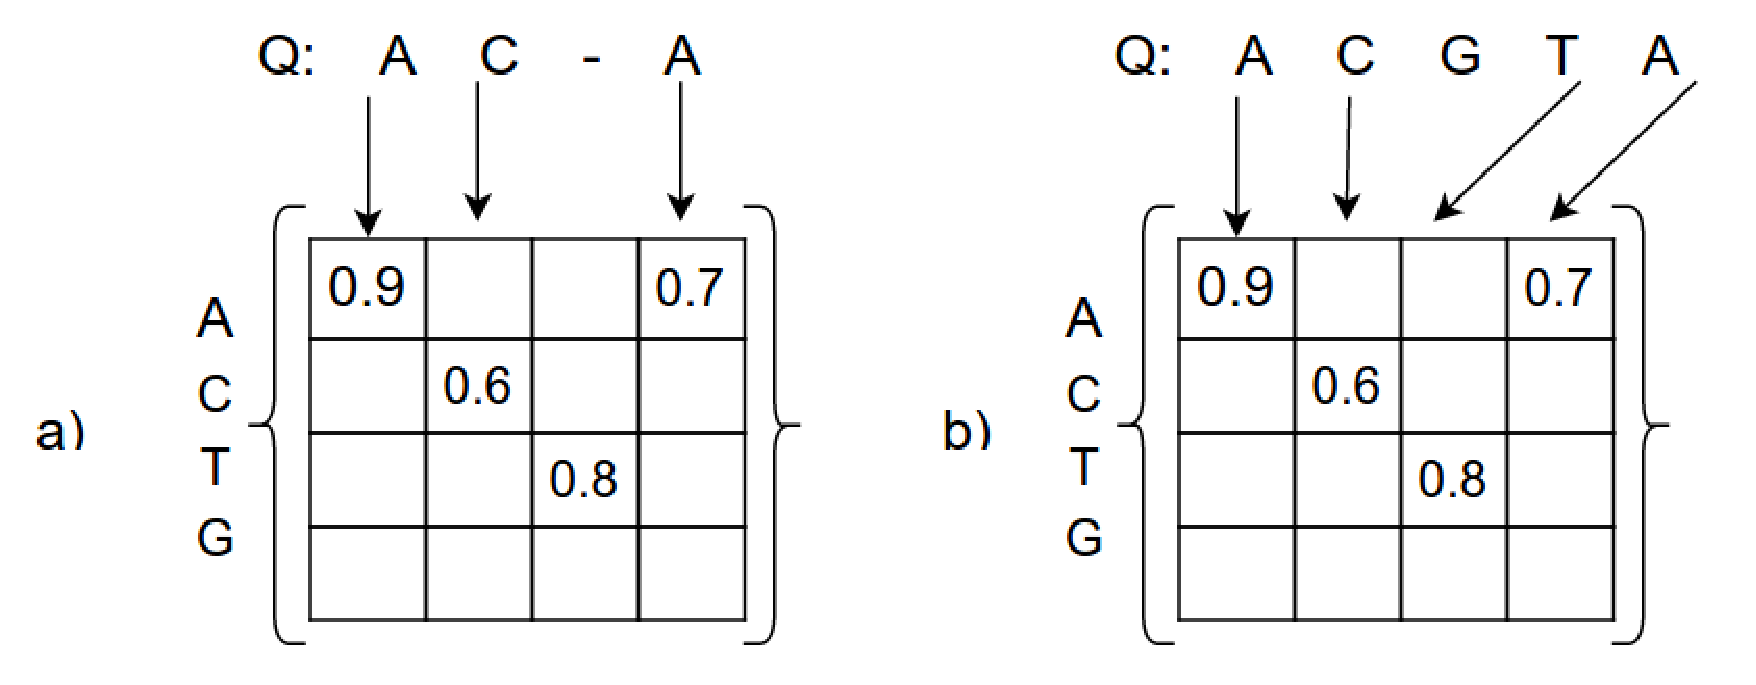
\includegraphics[scale=0.5]{indel}
    \caption{Proper alignment between $Q$ and $D$ showing a deletion (a) and an insertion (b).}
    \label{indel}
\end{figure*}

Before discussing this claim in detail, it is useful to first consider what an insertion or deletion means from a probabilistic genome. For the sake of this explanation, we assume $Q$ was generated by some unknown process from $D$. If we have an insertion into $Q$ then this new nucleotide would not be represented in $D$. Thus all nucleotides coming after the insertion will now point to the previous column of $D$ (see figure \ref{indel}b - shifts the distributions to the left). For a deletion in $Q$, a column of $D$ will now effectively never generate a nucleotide that is realized in $Q$. Thus all nuceotides coming after this deletion should be generated from the successor column in $D$ (see figure \ref{indel}a - shifts the distributions to the right). We can now view \"gaps\" as a device that shifts our distributions to try to best represent how the query sequence was generated.

Now instead of aligning a sequence to another sequence, we are aligning a deterministic sequence to a probabilistic sequence. Another way to phrase this is \"using the given scoring scheme, find the alignment that is most likely to have generated the query sequence.\" Let us consider the Needleman-Wunsch algorithm and provide an interpretation that holds for this problem. Figure \ref{NW} shows both the equation and visualization of the matrix. On one dimension we have the nucleotides forming $Q$, and along the other we have positions of $P$. 

***TODO: Make NW Figure ***

When we calculate scores we can interpret each part of the equations as follows:

\begin{description}
  \item[a)] Assume $q_j$ was generated from position $i$ of $P$.
  \item[b)] A deletion meaning position $i$ of $P$ never generated a realized nucleotide.
  \item[c)] An insertion meaning position $i$ has does not generate at this step (but may in the future).
\end{description}

The scoring scheme specifies that gaps should be allowed if it increases the likelihood of $Q$ by changing the positions nucleotides originated from.

We then return the gapped alignments as our matches. Note that multiple alignments may be returned and changing $w$ and $T$ will alter the sensitivity of ProbaBLAST similarily to how they do in BLAST.

\subsubsection{Choice of parameters}

We decided to play with different values of $T$ to see which one would generate the best results. Indeed, choosing a threshold value that is too high will result in too short matches, but a threshold that is too low could align the wrong nucleotides together.
For $w$, the length of the seed, we decided to go with $11$ as suggested in class, and is the default value in the standard nucleotide BLAST\footnote{BLAST FAQ: http://www.ncbi.nlm.nih.gov/blast/Why.shtml}.

\subsection{Model evaluation}

Evaluating ProbaBLAST's performance is perhaps the trickiest part of this project, as there is no \"ground truth\" to compare our results with. We opted for generating queries based on the probability distribution of the genome and added a few random indels and/or substitutions (each mutation type had a rate of 1\% to ensure they appeared). We generated many such queries, which we used as input to ProbaBLAST.

We suspected that query sequences of different lengths would perform differently using ProbaBLAST. We chose values of 25, 50, and 100 nucleotides for the queries. 

For each test query, we know that actual index it was generated from and use as the gold standard. When we run ProbaBLAST, we get back a list of matches as shown above. We consider a match correct, if our gold standard lies somewhere within the genome alignment of that match.

Using this method, there are two evaluation metrics we are interested in:

\begin{enumerate}
\item \emph{Precision} tells us the fraction of matches that match the gold standard.
\item \emph{Recall} tells us the fraction of test queries that were returned by ProbaBLAST.
\end{enumerate}

Ideally we want an algorithm with both high precision and recall. High recall means we return the correct sequence (but may return incorrect sequences as well). It easy easy to game this metric by predicting all possible alignments. Thus we need to balance recall with precision: a high precision means that we only returned matches that met the gold standard.

Note that this method has an inherent flaw. We assume that the gold standard is only possible place where the test sequence could have been generated from. But it very well could have been generated from somewhere else on the sequence. However, with longer sequences this should be less of a problem.

\section{Results}
 
\section{Discussion}

\subsection{Choice of index}

\subsection{Selecting the best threshold values}

\subsection{Length of test strings}


\begin{thebibliography}{9}

\bibitem{originalBLAST}
Altschul, S.F., Gish, W., Miller, W., Myers, E.W., Lipman, D.J. 
\emph{Basic local alignment search tool. }
Journal of Molecular Biology 215(3), 403–410 (1990).

\bibitem{blast2}
Ma J., Zhang L.
\emph{Modern BLAST Programs}
Problem Solving Handbook for Comput Biol. and Bioinformatics, pp.3-19, Springer, 2010.


\end{thebibliography}

\end{document}